\chapter{System Model}
\label{chp:system-model}
This chapter elaborates on the modeling aspects of the system being simulated. Having accurate models for both RF and Optical channels is essential for ensuring the reliability and performance of the simulation. These models provide a foundation for understanding and optimizing the system's behavior under various conditions.
\section{Network Model}
\label{sec:mod-ntw}
In this thesis, we consider an indoor hybrid network consisting of an RF network and an optical wireless network operating in parallel. In such a network, the user is connected to only one of the available networks at a particular time-instant, the user can switch between the networks when the management system initiates a vertical handover. Each of these networks consists of a single AP in the center of the simulation space. We consider a single user scenario for the purposes of the simulation, with the user starting at a random starting position on the receiver plane and moving through-out the simulation period based on the user mobility model defined in Section \ref{sec:mod-usr-mob}. The User Equipment (UE) is considered to have the appropriate receivers for both networks as defined in  Subsections \ref{subsec:mod-ntw-rf} and \ref{subsec:mod-ntw-optical} respectively.
\subsection{Wi-Fi Network Model}
\label{subsec:mod-ntw-rf}
A Single omnidirectional Wi-Fi AP is placed at the center of the room at ground level with the receiver plane. The Wi-Fi AP provides coverage to the entire simulation area. The receiver on the UE utilizes a single antenna system. To keep inter-cell interference at an undetectable level, the Wi-Fi network employs carrier sense multiple access/collision avoidance (CSMA/CA) similar to the system first presented in \cite{wu_novel_2020-1}. 
\subsection{Optical Network Model}
\label{subsec:mod-ntw-optical}
The optical network consists of one AP at the center of the simulation area, fixed at a height $h_{DL}=3m$. The AP is based on an “Array of Arrays model” proposed in \cite{sarbazi_tbs_2020} and \cite{kazemi_novel_2024}. It is a double tier architecture where vertical cavity surface emitting lasers are organized in matrices. The Ap consists of several such matrices specifically positioned and oriented to provide complete coverage to the simulation area.

\begin{figure}
    \centering
    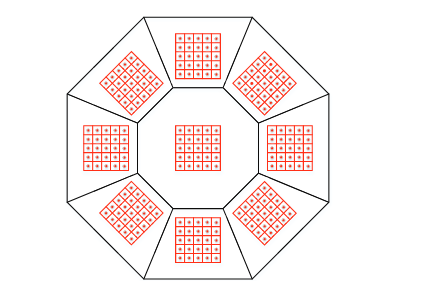
\includegraphics[width=0.75\linewidth]{Figures/Optical-AP-top-view.png}
    \caption{Double-tier access point architecture using array of arrays of VCSELs (top view). This design involves nine 5 × 5 VCSEL arrays \cite{sarbazi_tbs_2020}}
    \label{fig:mod-ntw-opt-top-view}
\end{figure}

 Each VCSEL emits a single optical beam which provides coverage to a small portion of the receiver plane. The AP consists of a total of $N_{VCSEL}=225$ VCSELs. These are distributed across 9 transmitter elements in a $3\times3$ grid with each element having $5\times5=25$ VCSELs. Figure \ref{fig:mod-ntw-opt-top-view} provides the top view of this two-tier AP design, while Figure \ref{fig:mod-ntw-opt-coverage} provides an overview of the network coverage with VCSEL to cell association. Lenses are utilized in front of each of the elements to separate the beam spots on the receiver plane and avoid significant overlap.

\begin{figure}
    \centering
    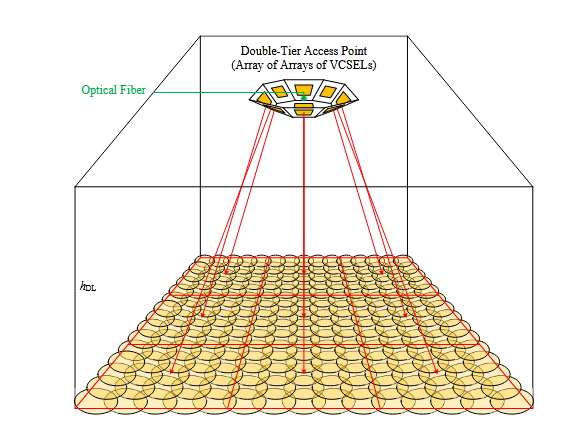
\includegraphics[width=0.75\linewidth]{Figures/Optical-AP-coverage.png}
\caption{Indoor grid-of-beam optical wireless multi-user access network using the proposed double-tier AP design based on an array of arrays of VCSELs \cite{kazemi_novel_2024}}
    \label{fig:mod-ntw-opt-coverage}
\end{figure}

The receiver on the UE utilizes the Photo-Diode (PD) matrix for detection. Utilizing photo-diodes for detection makes the system simple in design but does restrict the UE to a fixed orientation for consistent coverage. \cite{kazemi_novel_2024} utilizes an Angle Diversity receiver module on top of the PDs, consisting of 7 compound parabolic concentrators first proposed in \cite{sarbazi_design_2024}. For the purposes of managing the complexity of the simulation, we operate under the assumption that the receiver utilizes a simple PD matrix of a total area of $A_{PD}= 2cm^2$.
\section{Channel Model}
\label{sec:mod-channel}
\subsection{Wi-Fi Channel Model}
\label{subsec:mod-channel-rf}
\subsubsection{Channel Gain}
The channel gain for the link between the UE and the Wi-Fi AP represented by $ G_{WiFi}^u$ is given by  \cite{perahia_next_2013} as shown below in (\ref{eq:mod-wifi-gain}):
\begin{equation}
    G_{WiFi}^u = |H_{WiFI}^u|^210^{\frac{-L(d_u) + X_\sigma}{10}}.
    \label{eq:mod-wifi-gain}
\end{equation}
Where, $H_{WiFi}^u$ describes the channel transfer function; $X_\sigma$ represents the shadow fading. Finally, $L(.)$ represents the free space path loss.
\subsubsection{Channel transfer function}
The channel transfer function for the Wi-Fi channel $H_{WiFi}^u$  is given by a standard Rayleigh distribution, the PDF for which is given by (\ref{eq:mod-chn-wifi-transfer}) where $\sigma = 1$.
\begin{equation}
    f(x;\sigma )={\frac {x}{\sigma ^{2}}}\exp\left(-\frac{x^2}{2\sigma^2}\right),\quad x\geq 0.
    \label{eq:mod-chn-wifi-transfer}
\end{equation}
\subsubsection{Shadow fading}
Shadow fading for the Wi-Fi channel $X_\sigma$ is given by a Gaussian Random variable whose PDF is given by (\ref{eq:mod-chn-wifi-shadow}) where $\mu = 0$ and $\sigma = 10{dB}$.
\begin{equation}
    f(x) = \frac{1}{\sqrt{2\pi\sigma^2}} \exp\left(-\frac{(x - \mu)^2}{2\sigma^2}\right).
    \label{eq:mod-chn-wifi-shadow}
\end{equation}
\subsubsection{Free space path loss}
The free space path loss for the Wi-Fi channel $L(d)$ is given by (\ref{eq:mod-chn-wifi-path-loss}) where $f_c$ represents the central carrier frequency, while $d_{ref} = 10 \text{m}$ is the reference distance.
\begin{equation}
    L(d) = 
\begin{cases} 
20 \log_{10}(f_c d) - 147.5, & \text{if } d < d_{\text{ref}} \\
20 \log_{10}(f_c \frac{d^{2.75}}{d_{\text{ref}}^{1.75}}) - 147.5, & \text{if } d \geq d_{\text{ref}}
\end{cases}.
\label{eq:mod-chn-wifi-path-loss}
\end{equation}
\subsection{Optical Channel Model}
\label{subsec:mod-channel-optical}
\section{Performance Evaluation}
\label{sec:mod-perf}
\subsection{Wi-Fi Performance Evaluation}
\label{subsec:mod-perf-rf}
\subsubsection{SNR}
Based on the Wi-Fi channel model described in Section~\ref{subsec:mod-channel-rf} the SNR for the Wi-Fi user is given by (\ref{eq:mod-wifi-snr}) where the PSD of the noise at the receiver is represented by $N_{WiFi}=-174\space \text{dBM/Hz}$ while $B_{WiFi} = 20 \space \text{MHz}$ and $P_{WiFi}= 20 \space \text{dBm}$ represents the system bandwidth and the transmit power of Wi-Fi AP respectively.
\begin{equation}
    \gamma^{u}_{\text{WiFi}} = \frac{G^{u}_{\text{WiFi}} P_{\text{WiFi}}}{N_{\text{WiFi}} B_{\text{WiFi}}} .
    \label{eq:mod-wifi-snr}
\end{equation}
\subsubsection{Throughput}
Given the SNR, and utilizing the Shannon capacity as shown in \cite{wu_novel_2020-1} we calculate the throughput via (\ref{eq:mod-wifi-cap}) where $\zeta = 0.5$ is the effective utilization of the capacity which is impacted by the various overhead associated with transmission\cite{islam_throughput_2016}.
\begin{equation}
    r_u = \zeta * B \log_2(1 + \gamma_{WiFi}^u).
    \label{eq:mod-wifi-cap}
\end{equation}

\subsection{Optical Performance Evaluation}
\label{subsec:mod-perf-optical}
\subsubsection{SINR}
Assuming that all AP VCSELs are active and serving the user, the SINR is derived in \cite{sarbazi_tbs_2020} and given by (\ref{eq:mod-perf-optical-sinr}). Where, $R_{PD}$ represents the responsivity of the photodiode, and $h_i$ represents the channel DC Gain between the $i^{th}$ VCSEL and the user. $P_i$ represents the average electrical power previously given in () and, finally, $\sigma^2$ is the total noise variance of the system given in ().
\begin{equation}
    \gamma_i = \frac{R_{PD}^2h_i^2P_i}{\sum_{j\neq i}R_{PD}^2h_j^2P_j + \sigma^2}.
    \label{eq:mod-perf-optical-sinr}
\end{equation}

\subsubsection{Throughput}
Based on the work in \cite{sarbazi_tbs_2020}, the reliable transmission rate for each VCSEL is determined based on the Bit Error Rate (BER) performance. For the channel as described in Section \ref{subsec:mod-channel-optical}, A tight upper bound for the BER performance accurate to within 1 dB for $M\geq 4$ and $0 \leq \gamma_i \leq 30dB$ is given by ()\cite{goldsmith_variable-rate_1997}. Where M is the QAM size and $\gamma_i$ is the SINR of ${VECSEL}_i$ given by (\ref{eq:mod-perf-optical-sinr}).
\begin{equation}
    {BER} \leq 0.2\exp \left( \frac{1.5\gamma_i}{M - 1}\right).
    \label{eq:mod-perf-optical-ber}
\end{equation}
The highest order of the QAM constellation represented by $M_i$ is obtained by solving (\ref{eq:mod-perf-optical-ber}) with equality for $M_i$. This is represented by (\ref{eq:mod-perf-optical-mi}) where $\gamma_i$ represents SINR of ${VCSEL_i}$ and $\Gamma$ models the SINR gap given by (\ref{eq:mod-perf-optical-SINR gap}) which is specified by the forward error correction (FEC) limit\cite{sarbazi_tbs_2020}.
\begin{equation}
    M_i = 1 + \frac{\gamma_i}{\Gamma}.
    \label{eq:mod-perf-optical-mi}
\end{equation}

\begin{equation}
    \Gamma = \frac{-\ln{(5{BER})}}{1.5}.
    \label{eq:mod-perf-optical-SINR gap}
\end{equation}
The throughput of ${VCSEL_i}$ is given by (\ref{eq:mod-perf-optical-throughput}) where $B$ is the VCSEL bandwidth, $\zeta = \frac{N-2}{N}$ for $N$ being the number of sub-carriers in DCO-OFDM as described in \ref{subsec:mod-channel-optical} and $M_i$ given by (\ref{eq:mod-perf-optical-mi}).
\begin{equation}
    r_i = \zeta B \log_2M_i.
    \label{eq:mod-perf-optical-throughput}
\end{equation}
\section{User Mobility model}
\label{sec:mod-usr-mob}
User mobility is usually modeled based on popular stochastic models such as the Manhattan mobility model, reference point group mobility model \cite{kahn_experimental_1995} and the Random Waypoint Model (RWP) \cite{imielinski_dynamic_1996}. The RWP is a popular model widely utilized in the study of mobile ad hoc networks (MANETs) to simulate the movement patterns of mobile nodes. This model operates by having each node pause for a random period at a given location before selecting a new random destination within the simulation area. The node then travels towards this destination at a randomly chosen speed, which is uniformly distributed between a predefined minimum and maximum value. Upon reaching the destination, the node pauses again before repeating the process. This model is characterized by its simplicity and the ability to generate diverse mobility patterns. The original scenario for the RWP model was for large outdoor settings, with altering speeds when arriving at each waypoint. When adapting the model for indoor scenarios based on changes made by \cite{wu_smart_2020}, where the distance between waypoints is relatively short, the speed is considered to be constant for a short period. The movement within this period is considered an \textit{excursion}. Upon concluding the current excursion, the user selects a new speed, entirely uninfluenced by prior movements, and proceeds to continue traveling. Let $v$ denote the average speed. We assume the user's speed to be uniformly distributed between $0$ and $2v$. Figure \ref{fig:mod-user-mob} shows an example trace of the user movement on the simulator using RWP.
\begin{figure}
    \centering
    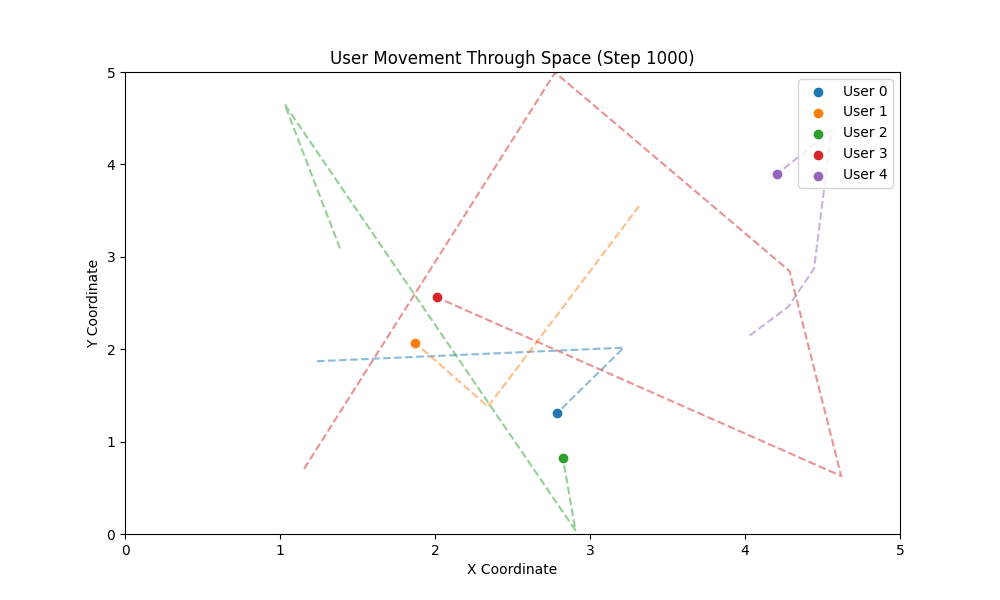
\includegraphics[width=1\linewidth]{Figures/mobility-plot-2025-04-28-15-30-46.png}
    \caption{User mobility simulation based on the RWP}
    \label{fig:mod-user-mob}
\end{figure}
\section{User localization}
\label{sec:mod-user-loc}
User localization is an essential pre-condition for a mobility-aware handover algorithm to operate effectively. The localization strategy varies based on the receiver and transmitter designs and the components used in the hybrid network. However, the handover algorithm itself is not intrinsically coupled to a specific strategy. The algorithm treats localization as a black box, from which it extracts the data it deems necessary for evaluation. As such, the handover algorithm can operate with any localization technique that satisfies the following criteria:
\begin{itemize}
    \item \textbf{Location accuracy:} The localization technique should provide accurate location information relative to the coverage area of an individual optical beam. The target is for the location estimation to be accurate enough for the algorithm to identify the individual optical beam that the user can be served by. For example, in our case with the transmitter design considerations, as the coverage area of an individual optical beam is $< 10 \text{cm}$, the localization strategy should be accurate enough in the cm scale.
    \item \textbf{Periodicity of measurements:} As further elaborated in \ref{chp:problem_statement}, the algorithm requires velocity and acceleration information for the decision-making process. If this information is being derived from the localization strategy itself, it is critical that the periodicity of the location estimation be frequent enough such that the derived quantities are accurate and up to date
\end{itemize}
Positioning techniques for indoor localization based on RF such as Wi-Fi, Bluetooth and Radio Frequency Identification (RFID) are not suitable candidates due to their low accuracy, high latency and hardware costs\cite{lin_real-time_2020}. Visible Light Positioning (VLP) has become significantly more attractive in this domain due to their low costs and high positioning accuracy. Studies have shown positional accuracy on the centimeter level\cite{hassan_indoor_2015}\cite{xu_experimental_2018}. Based on the receiving device, these positioning systems can be divided into two broad categories:
\begin{itemize}
    \item \textbf{Photo-diode based:} Low latency but sensitive to device rotation; positioning accuracy falls where UE does not have a fixed orientation
    \item \textbf{Image sensor based:} Robust to device rotation, but real-time performance limited. High computational load of image processing or communication latency due to transmission to server.
\end{itemize}
Taking in consideration the transmitter-receiver design as well the requirements of the handover algorithm itself, We decided to utilize a passive beam selection-based strategy first proposed in \cite{zeng_vcsel_2022}. The beam selection system utilizing Corner Cube Reflectors (CCR) offers low-power consumption and virtually no delay, enabling real-time tracking for high-speed users.
\subsection{Localization based on passive beam selection}
\label{subsec:mod-loc-pas-beam}
The VCSEL array system proposed by Zeng et al. in \cite{zeng_vcsel_2022} employs the signal strength strategy (SSS), which selects the optical beam with the highest received power. Each optical beam provides coverage to a specific area on the receiver plane. Thus, by considering the 3 optical beams with the highest received power, we can use triangulation to estimate the location of the user. The selection of the index of the beams to be utilized for this purpose can be formalized by (\ref{eq:mod-loc-1})
\begin{equation}
    \{I_1, I_2, I_3\} = \arg \max_{n \in N} \{{P_{rx,UE}^n}\}_{\text{top 3}}.
    \label{eq:mod-loc-1}
\end{equation}
Where \(I\) represents the index of the optical beam, \(N\) denotes the set of beams, and \(P_{r_{x,UE}}^n\) signifies the received optical power from the \(n\)-th beam. The strategy utilizes CCR to obtain a power matrix and then find the serving beam. Each VCSEL is associated with an RX element which detects any Reflected Signals (RS) associated with the user. Figure \ref{fig:mod-loc-ap} showcases the AP setup with the RX element associated with each VCSEL.
\begin{figure}
    \centering
    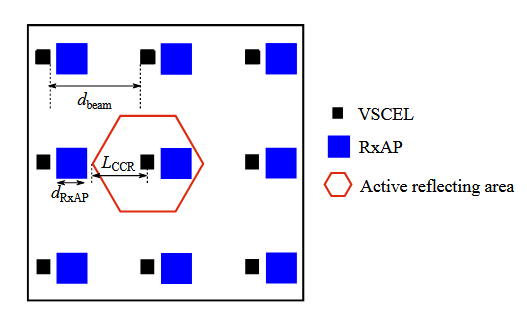
\includegraphics[width=0.75\linewidth]{Figures/modeling-localization-ap-design.png}
    \caption{The setup of AP using a CCR\cite{zeng_vcsel_2022}}
    \label{fig:mod-loc-ap}
\end{figure}

All beams send out a test signal simultaneously every set period. The UE sends back an (RS) which is received by the Rx APs. The optical beam selection is done according to (\ref{eq:mod-loc-1}), based on which location information is estimated. If the user is not connected to any optical beam, the optical beam with the highest power establishes connection and begins data transmission. Figure () provides an example of this operation in a system with 5 beams. 
\begin{figure}
    \centering
    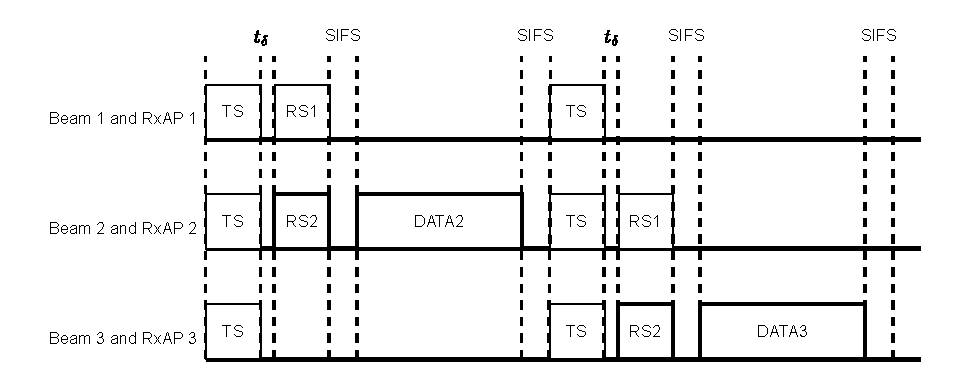
\includegraphics[width=\linewidth]{Figures/RF-OW-modeling-User localization.drawio.pdf}
    \caption{Beam selection mechanism}
    \label{fig:mod-loc-beam-ac}
\end{figure}
In the first period, All beams send a Test Signal (TS). The UE responds with an RS after a mean propagation delay of $t_\delta$. The optical beams for triangulation are first selected. The optical beam with the highest power (in this case, beam 2) then starts transmission after a Short Inter-Frame Space (SIFS). In the second period, again all the beams transmit a TS and the location estimation and beam selection procedure repeats (this time selecting beam 3).
The parameters for this selection criteria are shown in Table \ref{tab:mod-loc-params}.
\begin{table}[]
    \centering
    \begin{tabular}{|l|l|l|}
\hline
\textbf{Parameter}            & \textbf{Symbol}   & \textbf{Value}    \\ \hline
Test signal time              & $t_{TS}$          & 0.3 microseconds \\ \hline
Reflected signal time         & $t_{RS}$          & 0.3 microseconds \\ \hline
Average length of data packet\cite{khorov_tutorial_2019} & $L_{\text{Data}}$ & 64 kilobytes         \\ \hline
Mean propagation delay\cite{higgins_genetic_2009}        & $t_\delta$         & 3 nanoseconds    \\ \hline
SIFS\cite{khorov_tutorial_2019}                         & SIFS              & 2 microseconds   \\ \hline
\end{tabular}
    \caption{Parameters for beam selection\cite{zeng_vcsel_2022}}
    \label{tab:mod-loc-params}
\end{table}
\newline
\newline
In summary, the models developed and analyzed in this chapter provide a robust framework for understanding the underlying dynamics of the system, laying a solid foundation for the subsequent experimental validation and practical applications discussed in the following chapters